\begin{multicols}{2}
\textbf{Ingredients}
\begin{itemize}
\item 1 yellow onion \quad (45 kCal/ 1 gP/ 0 gF/ 11 gC)
\item 1 10 oz. bag of spinach \newline(70 kCal / 7 gP / 0 gF / 11 gC)
\item $\frac{1}{2}$ cup coconut milk \quad (276 kCal/ 3 gP/ 29 gF/ 7 gC)
\item 2 cans chickpeas \quad (840 kCal / 50 gP / 8 gF / 140 gC)
\item 1 28 oz. can crushed tomatoes \newline (175 kCal / 7 gP / 0 gF / 35 gC)
\item 2 cups basmati rice \quad (1,280 kCal / 32 gP / 0 gF / 280 gC)
\item 1 tbsp. olive oil \quad (119 kCal / 0 gP / 14 gF / 0 gC)
\item 1 tbsp. curry powder
\item 1 tbsp. minced garlic
\item 1 tsp. cumin
\item 1 tsp. grated ginger
\item $\frac{3}{4}$ tsp. salt 
\item $\frac{1}{2}$ coriander
\item 3 star anise pods
\item 7 green cardamom pods
\item 3 cups of water 


\end{itemize}


\columnbreak
\textbf{Procedure:}
\medskip


\begin{enumerate}
\item Mince onion, garlic, and ginger. Drain and rinse the chickpeas. 
\item Wash and rinse the rice. Crush cardamom pods to open them. Add anise, cardamom, and a sprinkle of cumin into the rice. Bring to a boil, then reduce to low heat and simmer for 13 minutes. Remove pods and anise before serving. 
\item In a large skillet, heat the oil over medium high heat. Add the onion and saute for 5 minutes. Add the garlic, ginger, and spinach and saute for 2 minutes until the spinach is fully wilted.
\item Carefully pour in the tomatoes, then add the curry powder, cumin, coriander, salt, and chickpeas. Cook for 5 minutes until bubbly.
\item Stir in the coconut milk until fully combined, then remove from the heat. Serve over rice.



\end{enumerate}
\begin{table}[H]
  \begin{center}
    \caption{Macro totals}
    \label{tab:table1}
    \begin{tabular}{c|c|c|c} % <-- Alignments: 1st column left, 2nd middle and 3rd right, with vertical lines in between
      \textbf{Calories} & \textbf{Protein} & \textbf{Fat} & \textbf{Carbs}\\
      \hline
      2,805 kCal & 100 g & 51 g & 484 g\\
    \end{tabular}
  \end{center}
\end{table}
\end{multicols}



\vspace{4mm}
\begin{center}
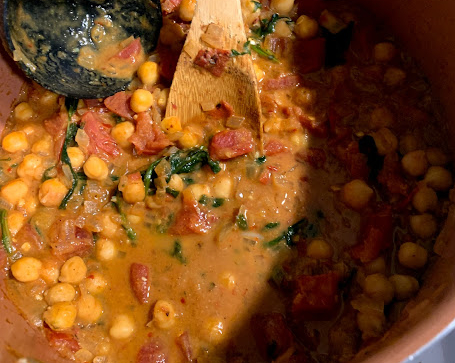
\includegraphics[scale=0.65]{Vegetarian Recipes/Coconut Chickpea Curry/chickpeacurry.jpg}
\end{center}